\chapter{First Design Iteration} \label{chapter:design-first-iteration}
Based on the insights gained through task and requirements analysis as well as the literature study, a first semi-interactive prototype was designed. The design consisted of the most important views needed for covering the version control workflow. Additionally, a simple editing view was integrated, so that the tasks for the user study could be embedded inside a realistic scenario. The overall interface was strongly influenced by existing code hosting platforms, such as Github \cite{_about_????}, Gitlab \cite{_code_????} and Bitbucket \cite{_bitbucket_????} as well as several Git GUIs \cite{_git_????}. The system can therefore be regarded as a crossbreed between version control and content authoring tool. How the system compares to a traditional version control system is described in more detail below.

\section{Comparison to Traditional VCSs} \label{sec:git-feature-comparison}
As compared to most other version control systems the interface only offers a minimal set of features. Some of them have been vastly simplified or adapted to the domain of language lesson authoring. A few features, such as the pull request and the history, are very close to their originals.

\begin{itemize}
  \item There is no differentiation between \emph{local and remote repositories} anymore. Church et al.'s \cite{church_case_2014} work has shown that hidden dependencies between these two often complicate matters for the user. Therefore, it was decided to have only one repository that is constantly up to date. This should, in theory, also simplify collaboration and avoid conflicts.
  \item Specifically \emph{tracking} files is not necessary. Every course or lesson that is created using the tool will be under version control.
  \item There is no \emph{staging} area anymore. As mentioned in chapter \ref{chapter:related-work} this feature is sometimes problematic and often inconvenient, because every change has to be staged before it can be saved (committed).
  \item The \emph{diff(erence)} view is presented by default before the user saves his or her changes. This ensures that the user knows what he or she is saving and provides an additional review mechanism. When using the Git CLI, diff is a separate command that needs to be executed when the user wants to look at what has changed.
  \item The diff view is enriched by a domain-specific design. It does not only display bare data as represented in the data format, but shows images, allows listening to sounds and visualizes boolean values, so that reviewing changes becomes simpler and is easier for users with a non-technical background.
  \item A \emph{pull request} feature (as on Github) was added. Because Git offers no formalized way of reviewing code before it is merged this feature enforces best practices. Furthermore, the requirements analysis has shown that reviewing new content that was produced by freelancers is very important.
  %\item Merging is always routed through a pull request, which allows users to review what has changed before merging branches. This reduced the abstraction as compared to merging only based on branch names.
  \item Visualizations were added in order to help users understand some of the more abstract concepts, such as branches. This was inspired by Bitbucket, which is using different visualizations to explain certain features.
\end{itemize}

As the reader might have noticed, the prototype still uses the original version control terminology (except for committing which is now called saving). This was done in order to learn which terms would cause most problems and to discuss this topic separately within a focus group following the first user study.

\section{Main Views}
Below, the most important screens of the prototype are shown. The version control features are always accessible at the top in a horizontal navigation bar. The content in the editing view (Figure \ref{fig:prot-initial-editor-view}) can be navigated by expanding a tree structure that also reflects the inherent composition of the content.

A typical user flow would consist of creating a new branch (Figure \ref{fig:create-branch}), editing some content (Figure \ref{fig:prot-initial-editor-view}), saving it (Figure \ref{fig:unsaved-changes}), optionally checking the edits in the history (Figure \ref{fig:history}) and finally creating a pull request (Figure \ref{fig:open-new-pr} and Figure \ref{fig:list-of-prs}).

\begin{figure}[h!]
 \centering
 \fbox{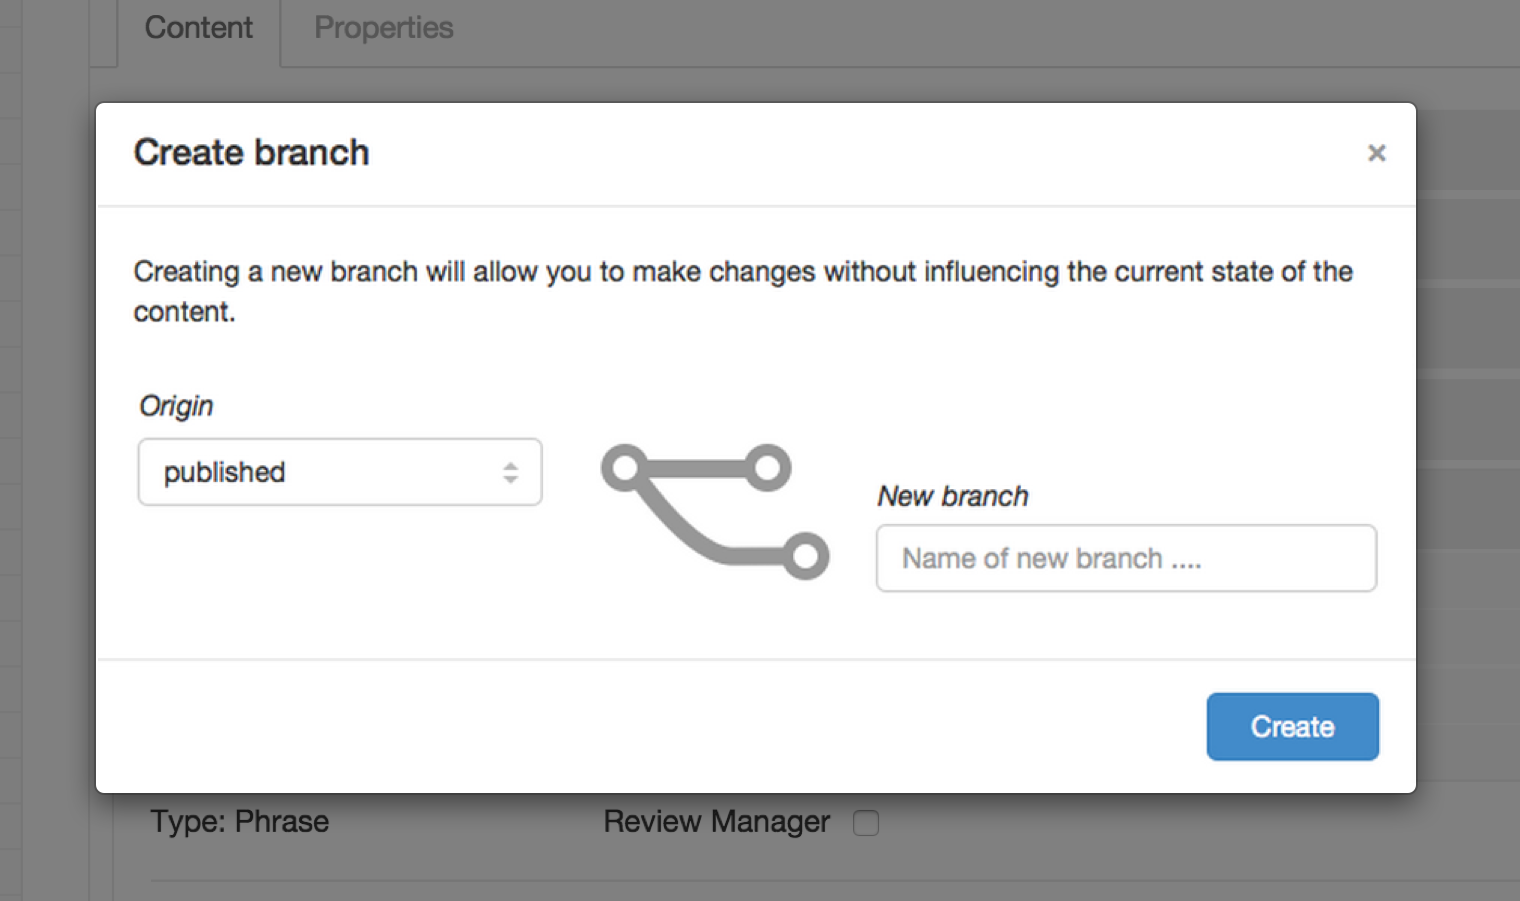
\includegraphics[width=\textwidth]{first-prototype/create-branch-modal}}
 \caption{Create Branch}
 \label{fig:create-branch}
\end{figure}


\begin{figure}[h!]
 \centering
 \fbox{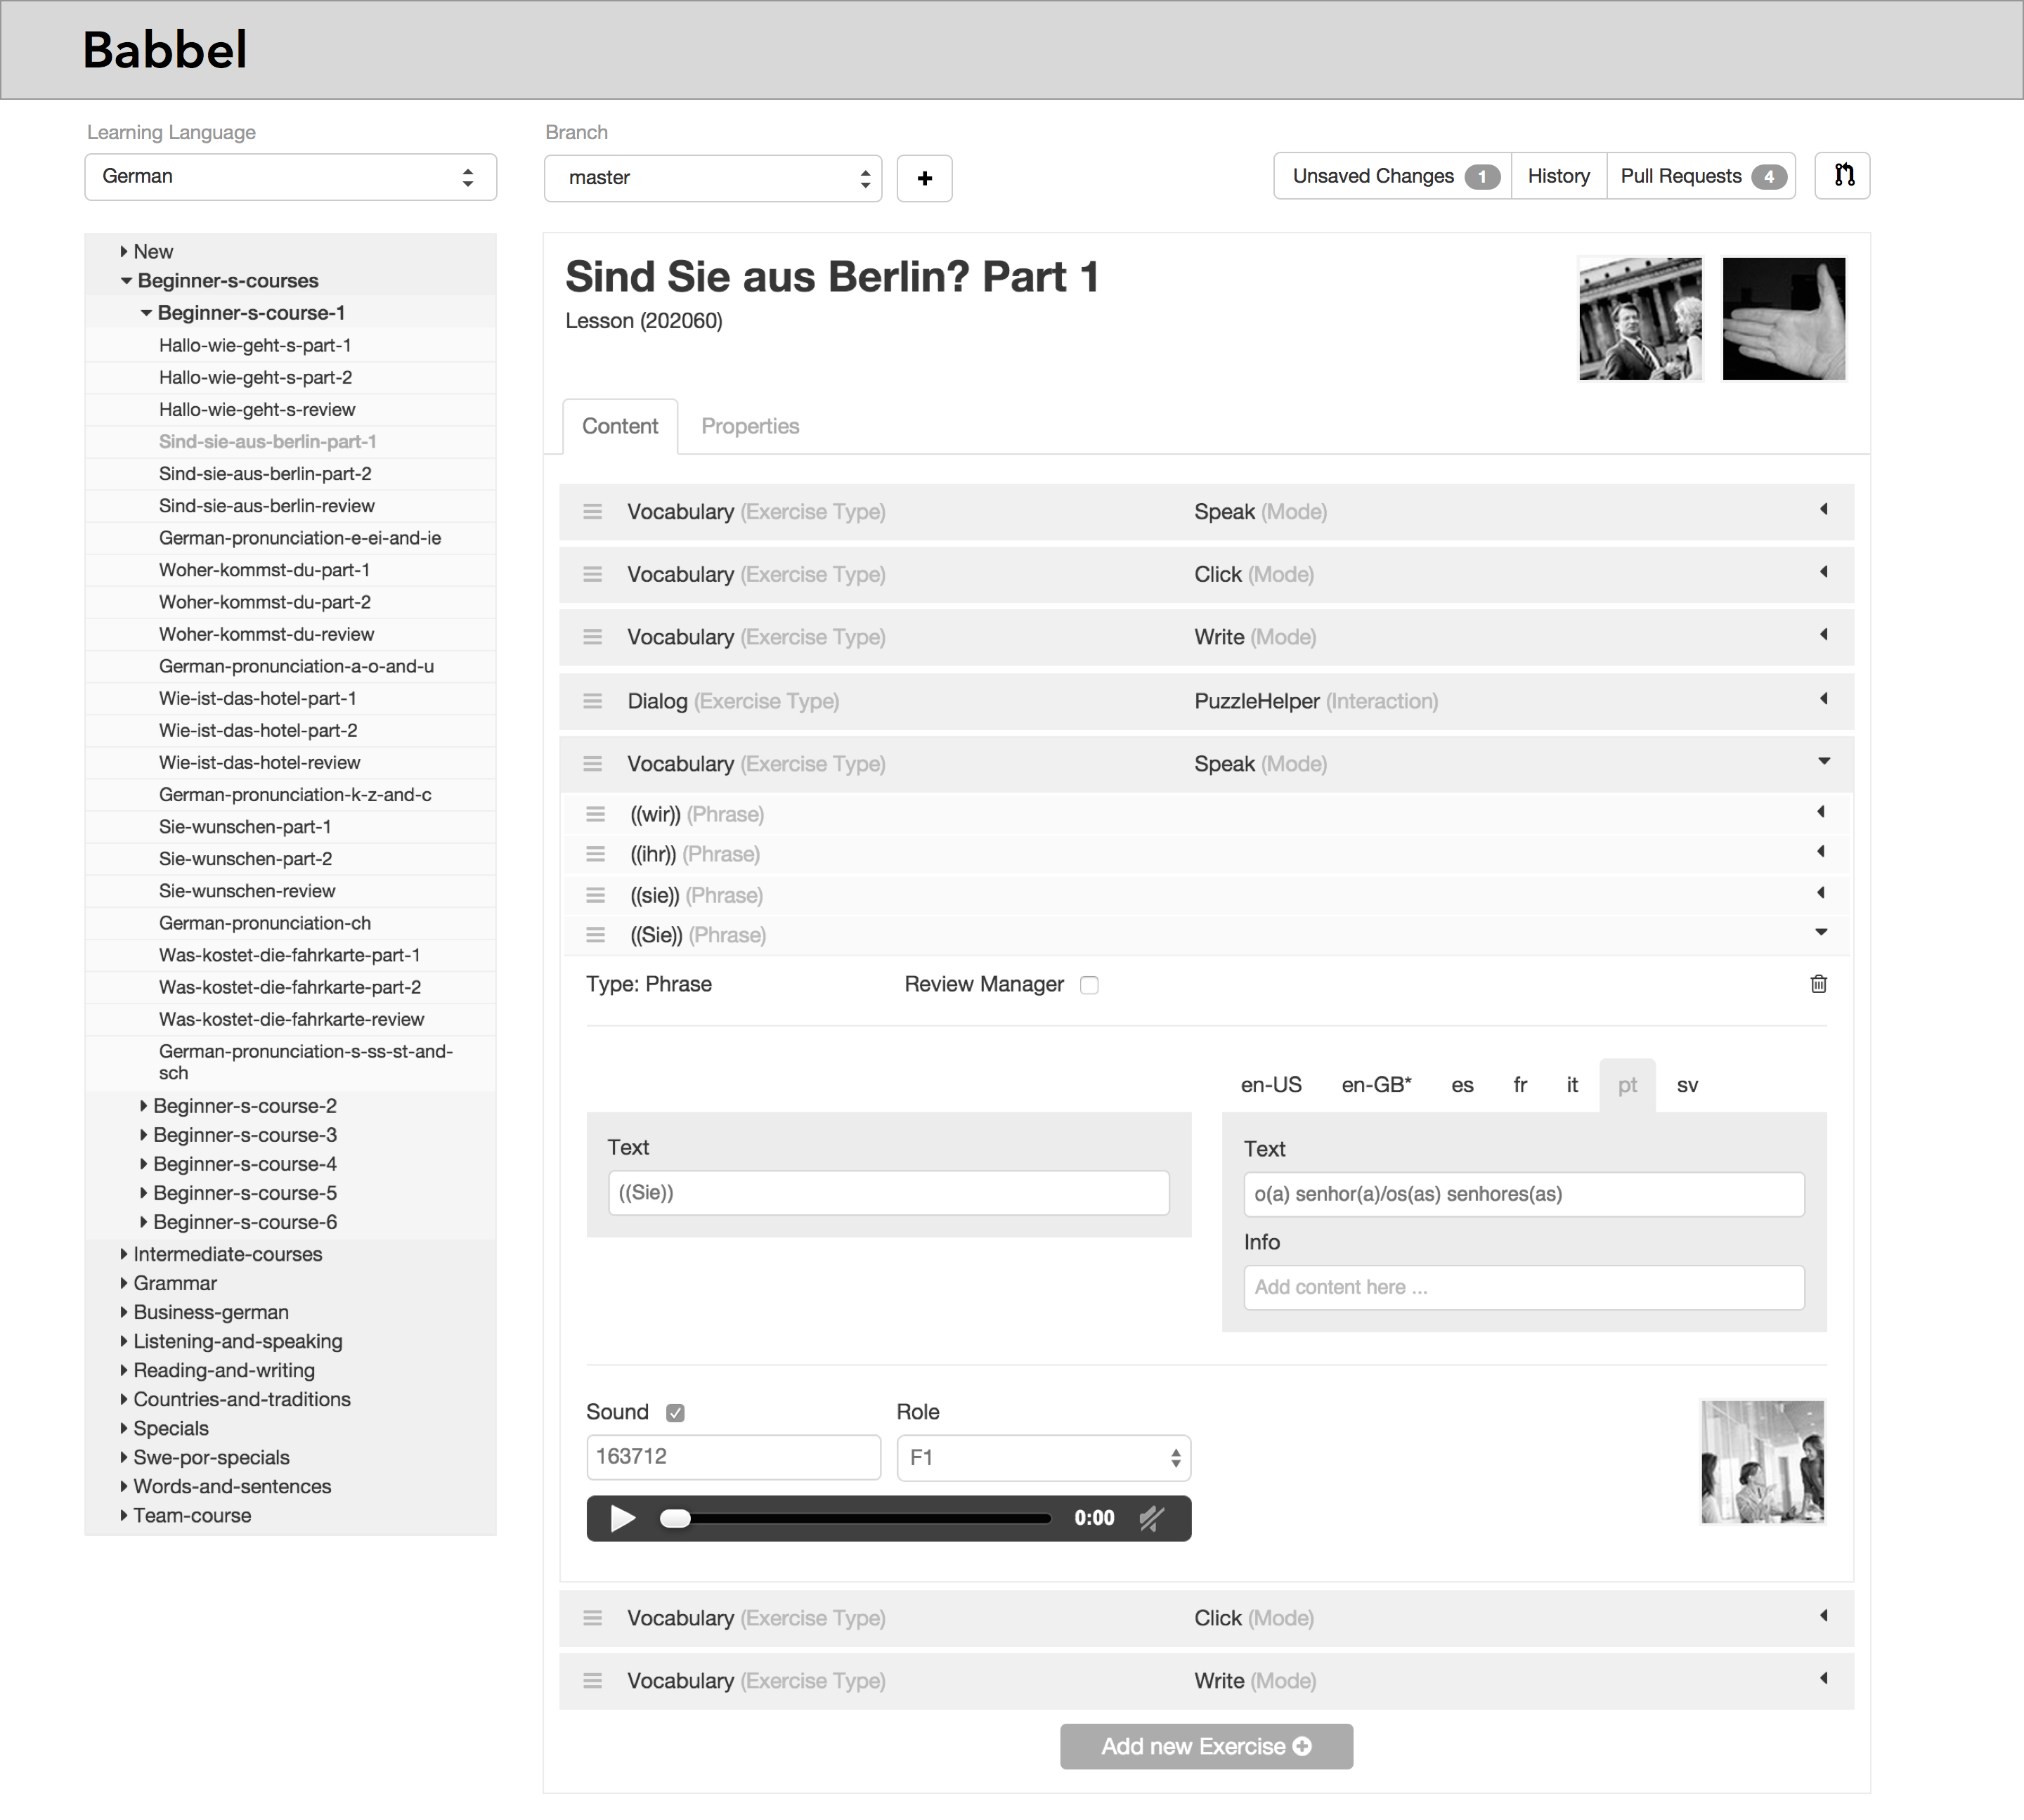
\includegraphics[width=\textwidth]{first-prototype/main-editing-view}}
 \caption{Editing View with Selected Lesson}
 \label{fig:prot-initial-editor-view}
\end{figure}

\begin{figure}[h!]
 \centering
 \fbox{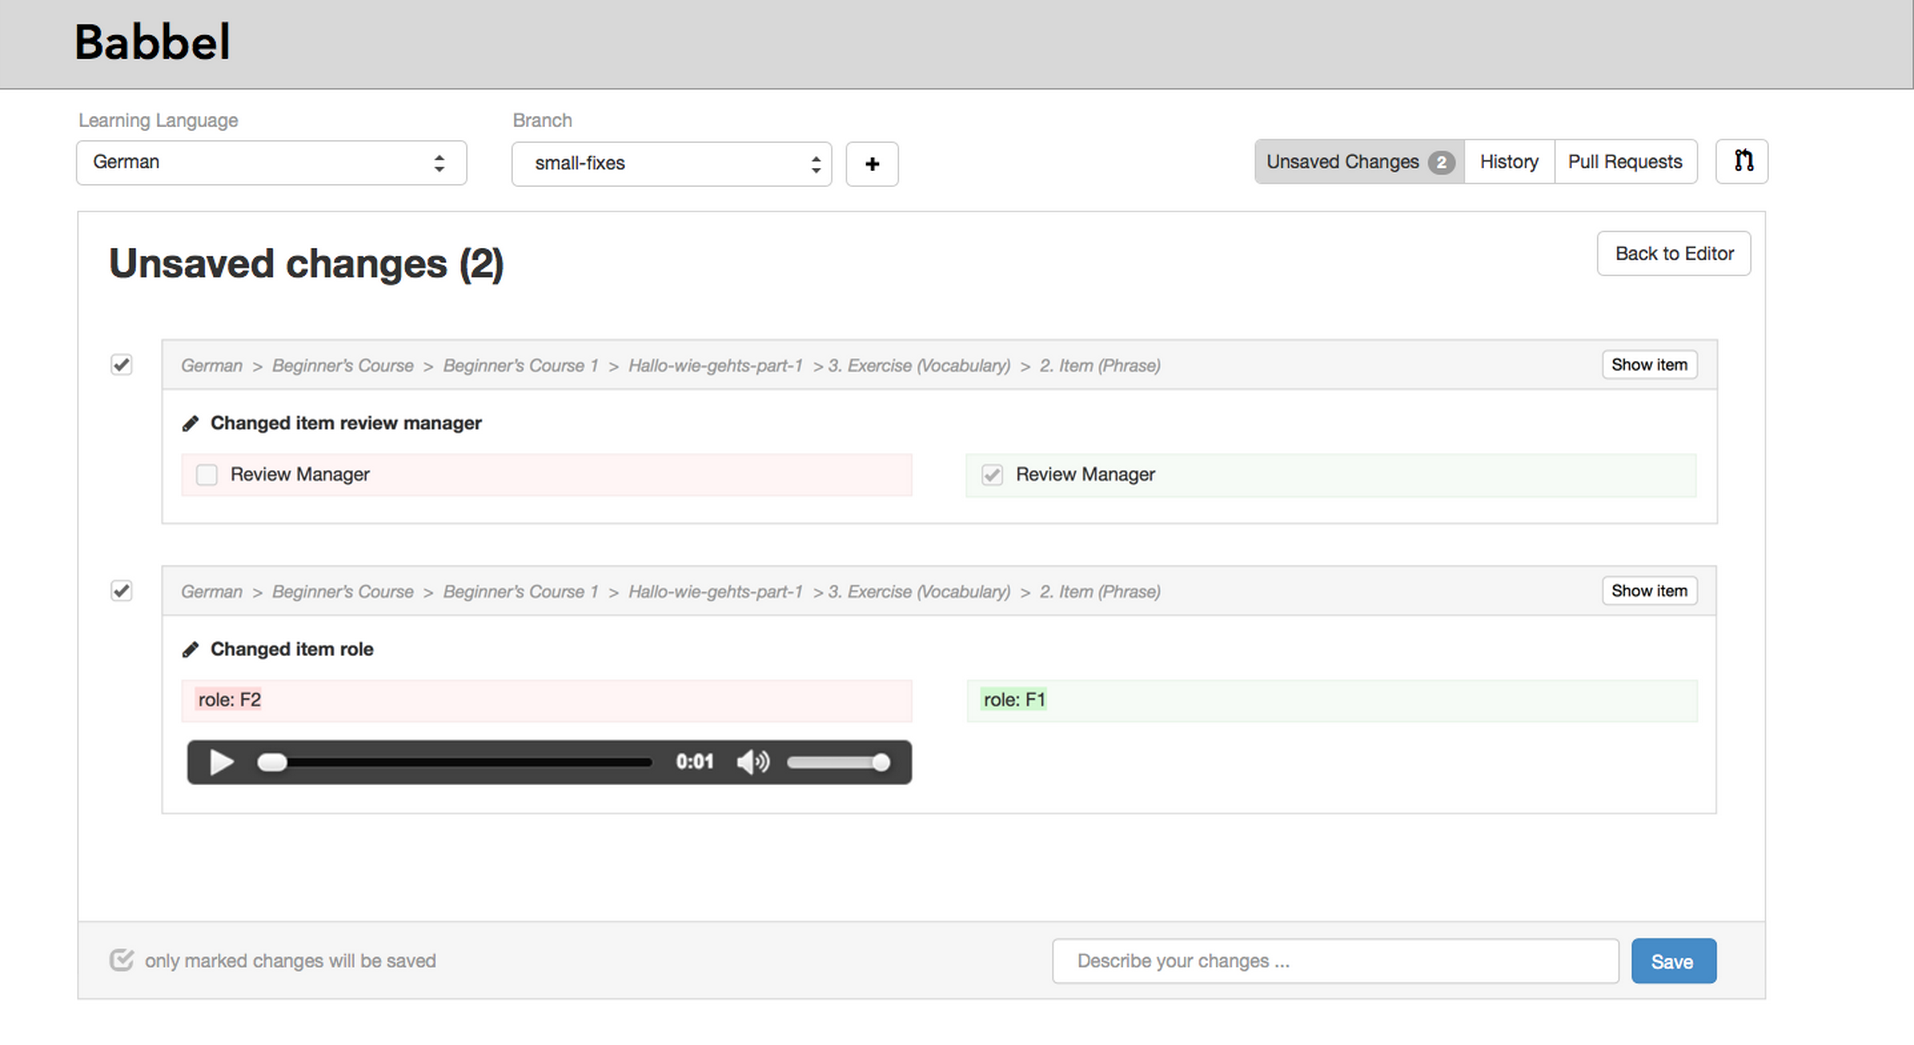
\includegraphics[width=\textwidth]{first-prototype/unsaved-changes}}
 \caption{Unsaved Changes / Diff view}
 \label{fig:unsaved-changes}
\end{figure}

\begin{figure}[h!]
 \centering
 \fbox{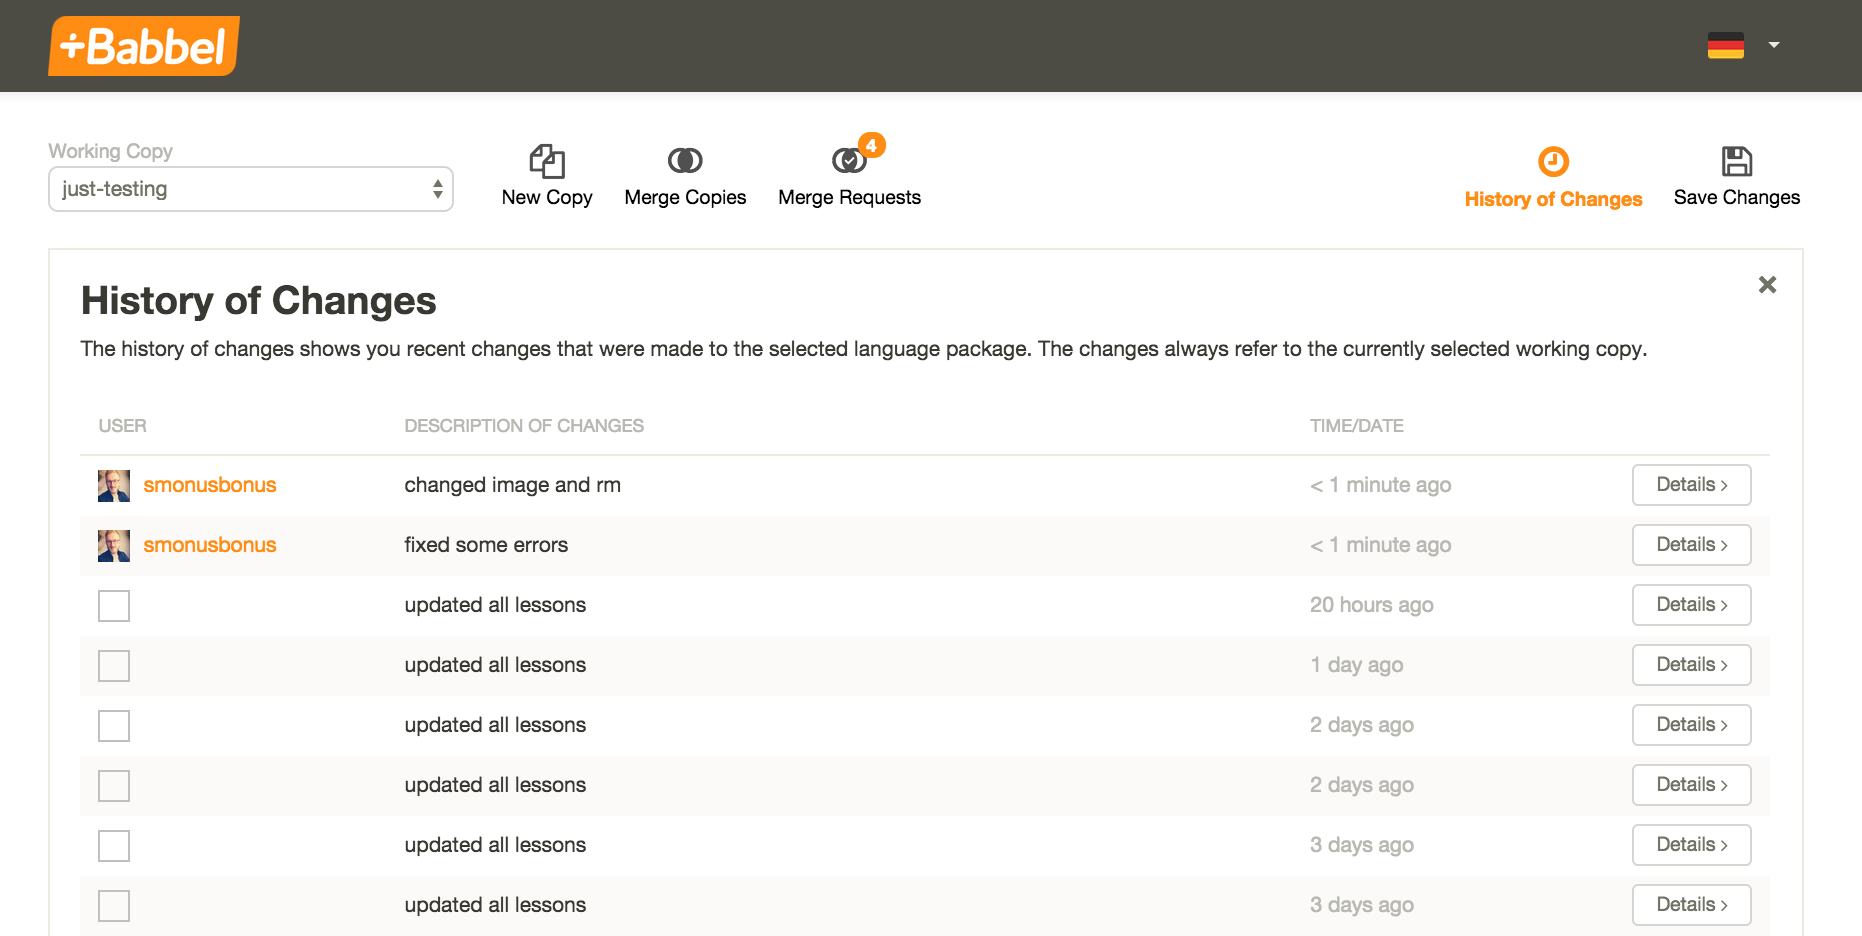
\includegraphics[width=\textwidth]{first-prototype/history}}
 \caption{History}
 \label{fig:history}
\end{figure}

\begin{figure}[h!]
 \centering
 \fbox{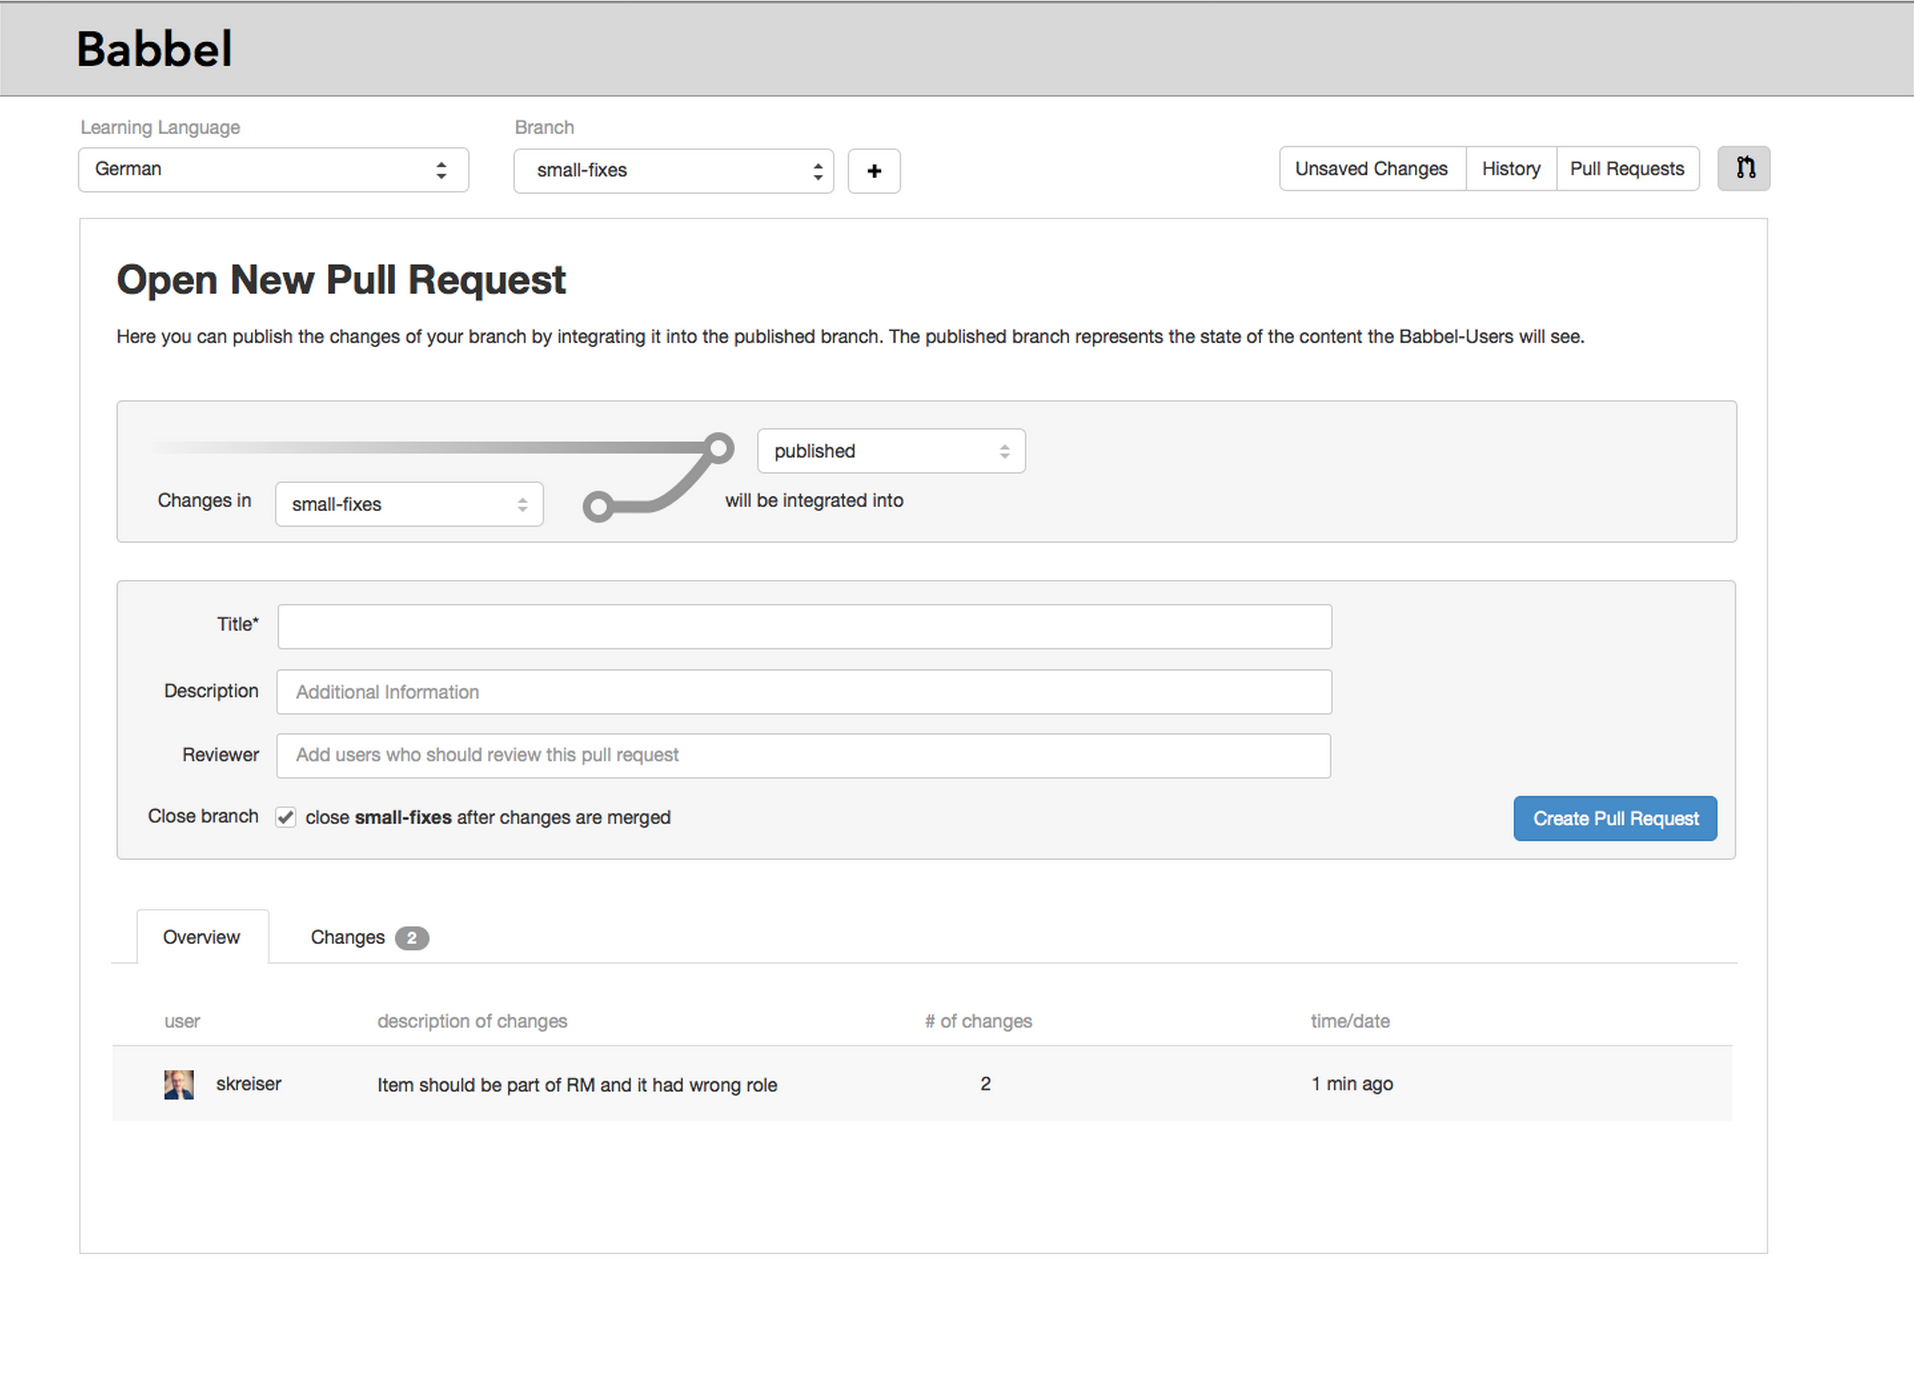
\includegraphics[width=\textwidth]{first-prototype/open-new-pr}}
 \caption{Create new pull request}
 \label{fig:open-new-pr}
\end{figure}

\begin{figure}[h!]
 \centering
 \fbox{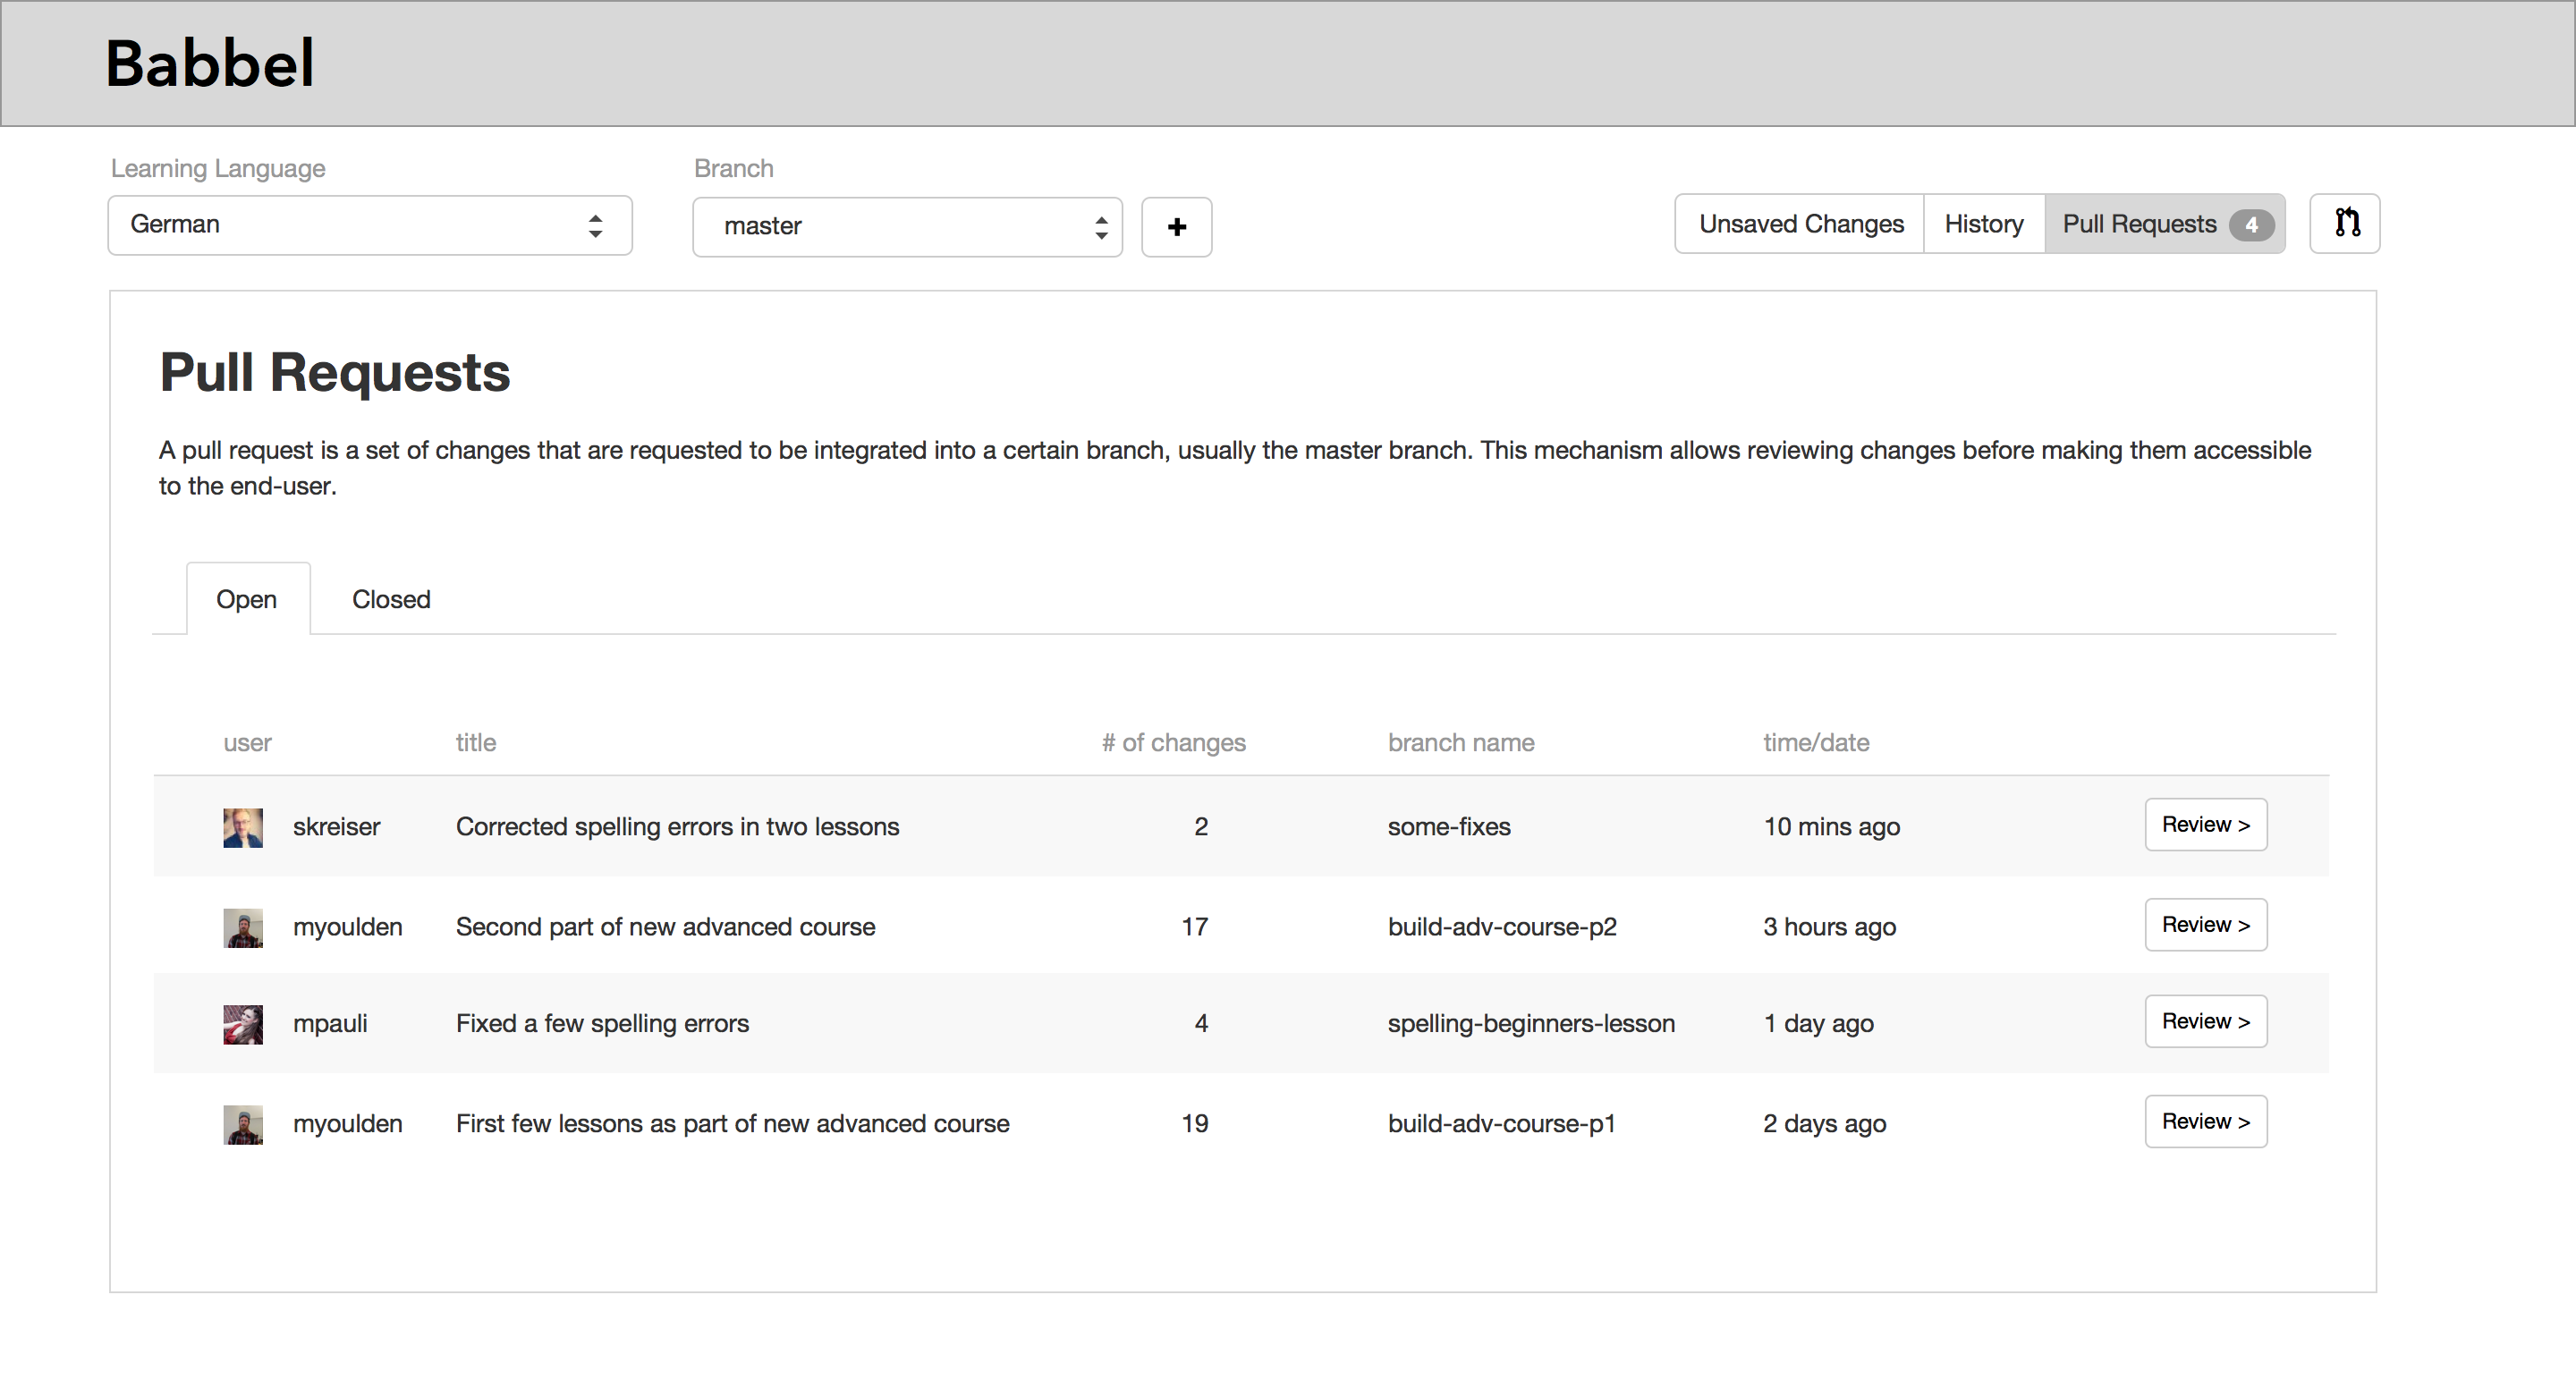
\includegraphics[width=\textwidth]{first-prototype/list-of-pull-requests}}
 \caption{List of pull requests}
 \label{fig:list-of-prs}
\end{figure}
